\documentclass[11pt,letterpaper]{article}
\usepackage[letterpaper,margin=0.85in,headheight=14pt]{geometry}
\usepackage{setspace,microtype,xcolor,parskip,enumitem,booktabs,array,longtable,fancyhdr,titlesec}
\usepackage[T1]{fontenc}
\usepackage{lmodern}
\usepackage[hidelinks]{hyperref}
\usepackage{tikz}
\usetikzlibrary{arrows.meta,positioning,shapes.geometric}

\setstretch{1.08}
\setlength{\parindent}{0pt}
\setlength{\parskip}{5pt}
\setlist[itemize]{leftmargin=1.55em,itemsep=2pt,topsep=3pt}
\setlist[enumerate]{leftmargin=1.7em,itemsep=3pt,topsep=3pt}
\titleformat{\section}{\normalfont\Large\bfseries}{\thesection}{0.6em}{}
\titleformat{\subsection}{\normalfont\large\bfseries}{\thesubsection}{0.6em}{}
\pagestyle{fancy}\fancyhf{}\renewcommand{\headrulewidth}{0pt}\fancyfoot[C]{\small\thepage}
\newcolumntype{L}[1]{>{\raggedright\arraybackslash}p{#1}}

\tikzset{
block/.style={draw,rounded corners=2pt,align=center,minimum height=.72cm,minimum width=2.15cm,font=\small},
smallblock/.style={draw,rounded corners=2pt,align=center,minimum height=.62cm,minimum width=1.8cm,font=\scriptsize},
arrow/.style={-{Latex[length=2mm]},thick},
dashedarrow/.style={-{Latex[length=2mm]},thick,dashed}
}

\begin{document}

\begin{center}
{\LARGE\bfseries Real-Time Collaborative Code Editor}\par
\vspace{5pt}
{\large\itshape Software Engineering Project Proposal}\par
\vspace{10pt}
{\normalsize Submitted by: Yuvraj Jasuja (1024030069) and Harwinder (1024030075)}\par
{\normalsize Department of Computer Engineering}\par
{\normalsize Thapar Institute of Engineering and Technology}\par
{\normalsize August 2026}
\end{center}
\vspace{7pt}\hrule\vspace{5pt}

\section{Higher-order Goal}
The goal of this project is to make collaborative programming more accessible and interactive by providing a shared environment where multiple users can work on the same code in real time.

Programming is often a collaborative activity. Students work together on assignments, developers pair program while solving problems, and teams frequently need to discuss and modify the same codebase. However, basic collaboration often involves repeatedly sharing files, copying code through messaging platforms, or manually merging different versions of the same program.

Our project aims to reduce this friction by creating a real-time coding environment in which users can join a common room and collaborate on the same code simultaneously.

\section{Introduction / Problem Statement}
Collaborative coding can become inefficient when multiple people are working on the same programming task.

Consider a common classroom situation where two students are solving a programming problem together. One student writes a part of the solution and sends the file to the other. The second student modifies it and sends another version back. As the number of changes increases, it becomes difficult to keep track of the latest version of the program.

This workflow creates several problems:
\begin{itemize}
\item Repeated sharing of source code files.
\item Multiple versions of the same program.
\item Difficulty identifying the latest version.
\item Delayed feedback between collaborators.
\item Version conflicts when different users modify the same code.
\item Lack of a simple shared environment for collaborative programming.
\end{itemize}

The Real-Time Collaborative Code Editor addresses this problem by allowing multiple users to join a shared coding room and view code changes as they happen.

\section{Objectives}
\begin{itemize}
\item Build a web-based platform for real-time collaborative code editing.
\item Allow users to create or join coding rooms using a unique Room ID.
\item Synchronize code changes between multiple connected users in real time.
\item Display active users currently connected to a coding room.
\item Provide a clean and interactive code editing environment.
\item Ensure that users joining an existing room can receive the current state of the code.
\item Extend the platform in future phases to support multiple programming languages and secure code execution.
\end{itemize}
\section{Methodology / Solution Approach}
\subsection{System Architecture}
The system follows a client-server architecture with real-time communication between users and the backend server.

The main components are:
\begin{itemize}
\item React-based user interface.
\item CodeMirror-based code editor.
\item Socket.IO for real-time communication.
\item Node.js and Express backend server.
\item Room-based communication for separate collaborative sessions.
\end{itemize}

\subsection{System Architecture Flow Diagram}
\begin{center}
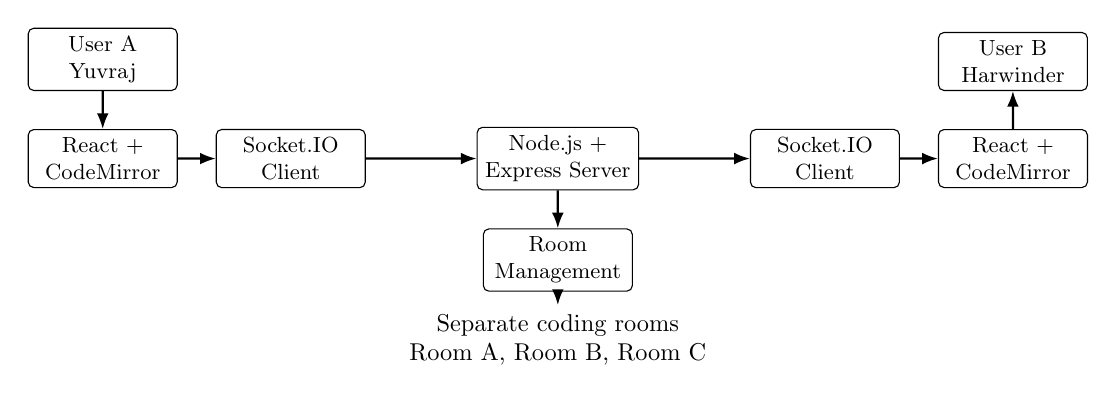
\begin{tikzpicture}[node distance=.55cm and .55cm,scale=.88,transform shape]
\node[block] (u1) {User A\\Yuvraj};
\node[block,below=of u1] (c1) {React +\\CodeMirror};
\node[block,right=of c1] (s1) {Socket.IO\\Client};
\node[block,right=1.6cm of s1] (server) {Node.js +\\Express Server};
\node[block,below=of server] (room) {Room\\Management};
\node[block,right=1.6cm of server] (s2) {Socket.IO\\Client};
\node[block,right=of s2] (c2) {React +\\CodeMirror};
\node[block,above=of c2] (u2) {User B\\Harwinder};
\draw[arrow] (u1)--(c1);
\draw[arrow] (c1)--(s1);
\draw[arrow] (s1)--(server);
\draw[arrow] (server)--(s2);
\draw[arrow] (s2)--(c2);
\draw[arrow] (c2)--(u2);
\draw[arrow] (server)--(room);
\draw[dashedarrow] (room)--++(0,-.65) node[below,align=center]{Separate coding rooms\\Room A, Room B, Room C};
\end{tikzpicture}
\end{center}

The browser contains the React interface and CodeMirror editor. Socket.IO maintains the real-time connection with the Node.js and Express server. The server manages room membership and broadcasts changes to users in the same room.

\subsection{Real-Time Collaboration Flow}
The main workflow is:
\begin{enumerate}
\item A user enters a username and creates a new coding room or enters an existing Room ID.
\item The user establishes a Socket.IO connection with the backend server.
\item The server associates the user with the requested coding room.
\item Other users join the same room using the Room ID.
\item When a user modifies the code, CodeMirror detects the change.
\item The updated code is emitted to the backend using Socket.IO.
\item The server broadcasts the update to other users in the same room.
\item Connected users receive the update and their editor reflects the new code.
\item When a user disconnects, the server notifies the remaining users.
\end{enumerate}

\subsection{Real-Time Code Synchronization Flow Diagram}
\begin{center}
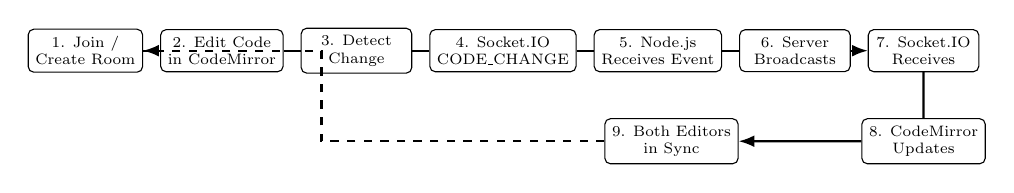
\begin{tikzpicture}[node distance=.28cm,scale=.78,transform shape]
\node[smallblock] (a) {1. Join /\\Create Room};
\node[smallblock,right=of a] (b) {2. Edit Code\\in CodeMirror};
\node[smallblock,right=of b] (c) {3. Detect\\Change};
\node[smallblock,right=of c] (d) {4. Socket.IO\\CODE\_CHANGE};
\node[smallblock,right=of d] (e) {5. Node.js\\Receives Event};
\node[smallblock,right=of e] (f) {6. Server\\Broadcasts};
\node[smallblock,right=of f] (g) {7. Socket.IO\\Receives};
\node[smallblock,below=.75cm of g] (h) {8. CodeMirror\\Updates};
\node[smallblock,left=2cm of h] (i) {9. Both Editors\\in Sync};
\draw[arrow](a)--(b)--(c)--(d)--(e)--(f)--(g);
\draw[arrow](g)--(h)--(i);
\draw[dashedarrow](i)--++(-5.7cm,0)|-(a);
\end{tikzpicture}
\end{center}

This diagram shows the core operation: a change made by one user is detected, transmitted through Socket.IO, processed by the Node.js server, broadcast to room members, and reflected in the other editor.

\subsection{Room-Based Communication}
Each collaborative session is organized as a separate room. This prevents code changes from one group of users from being sent to unrelated users.

For example:
\begin{itemize}
\item Room A may contain Yuvraj and Harwinder.
\item Room B may contain other users.
\end{itemize}

Code changes generated inside Room A are only broadcast to users connected to Room A.

\subsection{Future Multi-Language Execution}
The current version focuses primarily on real-time collaborative editing. A future extension will allow users to select languages such as C++, Java, Python, JavaScript, and C.

Users will be able to write code, provide input, execute the program, and view output or compilation errors. Because arbitrary code should not be executed directly on the main application server, execution will use a secure sandbox or external execution service.

\begin{center}
\textbf{Code Editor $\rightarrow$ Secure Sandbox / Execution API $\rightarrow$ Compiler / Runtime $\rightarrow$ Output}
\end{center}



\subsection{User Journey Flow Diagram}

The following flow represents the complete journey of a user from opening the application to collaborating inside a coding room.

\begin{center}
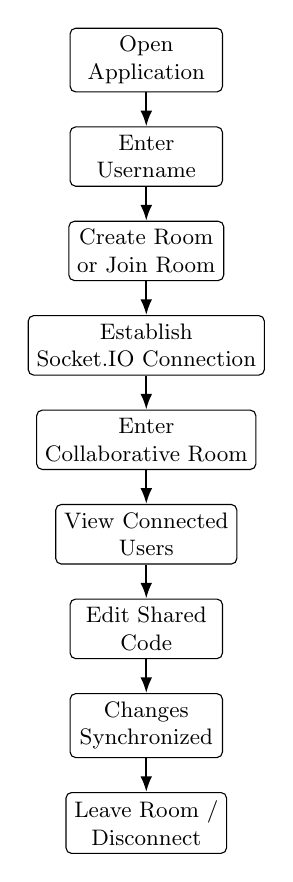
\begin{tikzpicture}[node distance=.48cm and .42cm,scale=.9,transform shape]
\node[block] (start) {Open\\Application};
\node[block,below=of start] (name) {Enter\\Username};
\node[block,below=of name] (choice) {Create Room\\or Join Room};
\node[block,below=of choice] (connect) {Establish\\Socket.IO Connection};
\node[block,below=of connect] (room) {Enter\\Collaborative Room};
\node[block,below=of room] (users) {View Connected\\Users};
\node[block,below=of users] (edit) {Edit Shared\\Code};
\node[block,below=of edit] (sync) {Changes\\Synchronized};
\node[block,below=of sync] (leave) {Leave Room /\\Disconnect};

\draw[arrow](start)--(name);
\draw[arrow](name)--(choice);
\draw[arrow](choice)--(connect);
\draw[arrow](connect)--(room);
\draw[arrow](room)--(users);
\draw[arrow](users)--(edit);
\draw[arrow](edit)--(sync);
\draw[arrow](sync)--(leave);
\end{tikzpicture}
\end{center}

This flow gives a simple view of the user's interaction with the system. The user first enters the application, joins a room, connects to the real-time server, and then collaborates through the shared editor.

\subsection{Client--Server Communication Flow}

The project uses event-based communication between the browser and the backend server. The simplified communication sequence is shown below.

\begin{center}
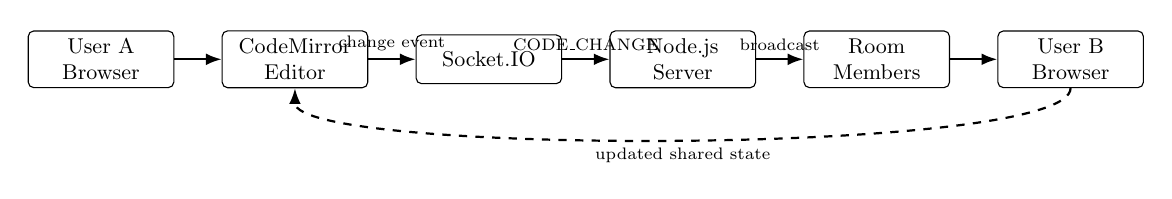
\begin{tikzpicture}[node distance=.55cm and .7cm,scale=.86,transform shape]
\node[block] (client1) {User A\\Browser};
\node[block,right=of client1] (editor) {CodeMirror\\Editor};
\node[block,right=of editor] (socket) {Socket.IO};
\node[block,right=of socket] (server) {Node.js\\Server};
\node[block,right=of server] (room) {Room\\Members};
\node[block,right=of room] (client2) {User B\\Browser};

\draw[arrow](client1)--(editor);
\draw[arrow](editor)--node[above,font=\scriptsize]{change event}(socket);
\draw[arrow](socket)--node[above,font=\scriptsize]{CODE\_CHANGE}(server);
\draw[arrow](server)--node[above,font=\scriptsize]{broadcast}(room);
\draw[arrow](room)--(client2);

\draw[dashedarrow] (client2.south) .. controls +(0,-1.0) and +(0,-1.0) .. node[below,font=\scriptsize]{updated shared state} (editor.south);
\end{tikzpicture}
\end{center}

The important point is that the server does not need to continuously refresh the browser. Instead, the Socket.IO connection allows events to be sent as soon as a change occurs.

\subsection{Room Isolation Flow Diagram}

Room isolation ensures that a collaboration session remains separate from other sessions.

\begin{center}
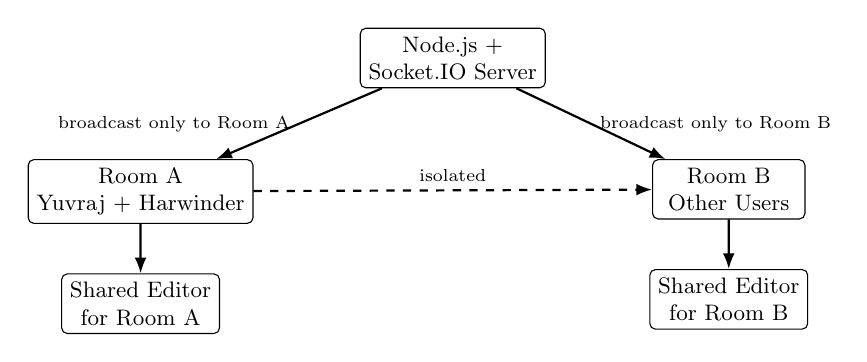
\begin{tikzpicture}[node distance=.7cm and .8cm,scale=.9,transform shape]
\node[block] (server) {Node.js +\\Socket.IO Server};

\node[block,below left=1.0cm and 1.5cm of server] (ra) {Room A\\Yuvraj + Harwinder};
\node[block,below right=1.0cm and 1.5cm of server] (rb) {Room B\\Other Users};

\node[block,below=of ra] (ea) {Shared Editor\\for Room A};
\node[block,below=of rb] (eb) {Shared Editor\\for Room B};

\draw[arrow](server)--node[left,font=\scriptsize]{broadcast only to Room A}(ra);
\draw[arrow](server)--node[right,font=\scriptsize]{broadcast only to Room B}(rb);
\draw[arrow](ra)--(ea);
\draw[arrow](rb)--(eb);

\draw[dashedarrow] (ra) -- node[above,font=\scriptsize]{isolated} (rb);
\end{tikzpicture}
\end{center}

A change generated in Room A is distributed only to the users belonging to Room A. Similarly, Room B remains independent. This room-based design allows several coding sessions to operate at the same time.

\subsection{Future Code Execution Flow Diagram}

The collaborative editor can later be extended into a multi-language online coding platform. The planned execution path is shown below.

\begin{center}
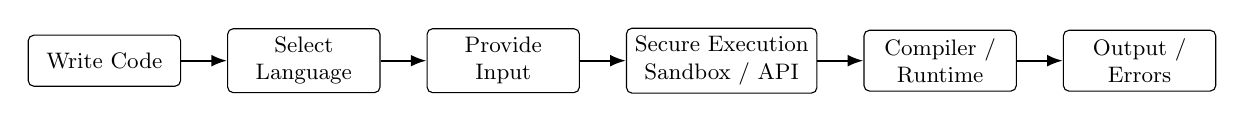
\begin{tikzpicture}[node distance=.62cm and .65cm,scale=.9,transform shape]
\node[block] (code) {Write Code};
\node[block,right=of code] (lang) {Select\\Language};
\node[block,right=of lang] (input) {Provide\\Input};
\node[block,right=of input] (api) {Secure Execution\\Sandbox / API};
\node[block,right=of api] (compile) {Compiler /\\Runtime};
\node[block,right=of compile] (result) {Output /\\Errors};

\draw[arrow](code)--(lang);
\draw[arrow](lang)--(input);
\draw[arrow](input)--(api);
\draw[arrow](api)--(compile);
\draw[arrow](compile)--(result);
\end{tikzpicture}
\end{center}

This is a planned extension rather than a claim about the current implementation. The execution component will be isolated from the main application server so that arbitrary user programs are not executed directly on the collaboration server.

\subsection{Deployment Flow Diagram}

The application can be deployed as a web service so that collaborators can access the same coding room from different systems.

\begin{center}
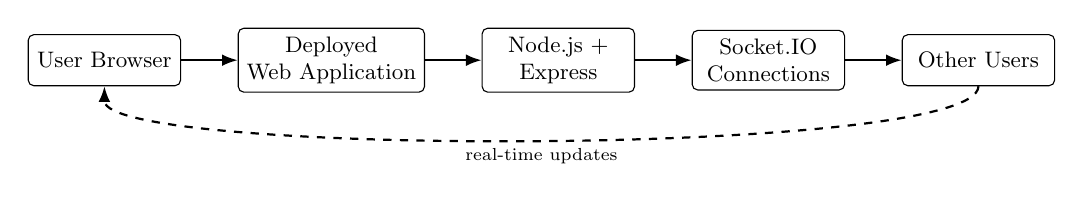
\begin{tikzpicture}[node distance=.7cm and .8cm,scale=.9,transform shape]
\node[block] (a) {User Browser};
\node[block,right=of a] (b) {Deployed\\Web Application};
\node[block,right=of b] (c) {Node.js +\\Express};
\node[block,right=of c] (d) {Socket.IO\\Connections};
\node[block,right=of d] (e) {Other Users};

\draw[arrow](a)--(b);
\draw[arrow](b)--(c);
\draw[arrow](c)--(d);
\draw[arrow](d)--(e);
\draw[dashedarrow] (e.south) .. controls +(0,-1.0) and +(0,-1.0) .. node[below,font=\scriptsize]{real-time updates} (a.south);
\end{tikzpicture}
\end{center}

Deployment allows the same collaborative environment to be accessed over the internet rather than only from a local development machine.


\section{Tech Stack}
\begin{itemize}
\item \textbf{React:} Frontend user interface.
\item \textbf{CodeMirror:} Interactive code editing environment.
\item \textbf{Socket.IO:} Real-time, bidirectional communication.
\item \textbf{Node.js:} Backend runtime.
\item \textbf{Express.js:} Backend server and routes.
\item \textbf{UUID:} Unique Room ID generation.
\item \textbf{Render:} Possible deployment platform.
\end{itemize}

\newpage
\section{Evaluation Criteria}
\begin{itemize}
\item \textbf{Synchronization Accuracy:} Code changes are correctly reflected for users in the same room.
\item \textbf{Real-Time Response:} Low delay between editing and receiving updates.
\item \textbf{Room Isolation:} Users in different rooms do not receive unrelated updates.
\item \textbf{Connection Handling:} Correct join and disconnect behavior.
\item \textbf{Concurrent Users:} Ability to support multiple users in a shared room.
\item \textbf{Usability:} Users can easily create, join, and use a room.
\end{itemize}

\section{Scalability}
The architecture is based on independent real-time rooms. Potential improvements include multiple backend instances, a distributed Socket.IO adapter, persistent project storage, database support, and a separate code execution service.

\section{Resources / Tooling}
\begin{itemize}
\item React and JavaScript for frontend development.
\item CodeMirror for the coding interface.
\item Node.js and Express for backend development.
\item Socket.IO for real-time communication.
\item GitHub for version control and project management.
\item Render or another cloud platform for deployment.
\item Secure execution API or sandbox for future code execution.
\end{itemize}


\section{Project Scope and Deliverables}
\subsection{Initial Deliverable}
\begin{itemize}
\item Home page for username and Room ID.
\item Create a unique coding room.
\item Join an existing coding room.
\item Real-time collaborative code editing.
\item Connected-user display.
\item Room-based Socket.IO communication.
\item User connection and disconnection handling.
\end{itemize}

\subsection{Subsequent Deliverables}
\begin{itemize}
\item Multiple programming language support.
\item Language-based syntax highlighting.
\item Run code functionality.
\item Custom input and output terminal.
\item Compilation and runtime error display.
\item Execution time information.
\item User authentication.
\item Saving and loading projects.
\item Multi-file project support.
\item Live cursor tracking.
\item Integrated collaborative chat.
\end{itemize}

\section{Risks and Mitigations}
\begin{itemize}
\item \textbf{Synchronization conflicts:} Future versions can use operational transformation or CRDT-based collaboration for more advanced concurrent editing.
\item \textbf{Network latency:} Socket.IO reconnection support can improve reliability.
\item \textbf{User disconnection:} Disconnect events update the active-user list.
\item \textbf{Unauthorized room access:} Future authentication and private-room controls can be added.
\item \textbf{Code execution security:} Future execution will use an isolated sandbox or execution service.
\end{itemize}

\section{Timeline}
\begin{center}
\small
\begin{tabular}{@{}L{0.18\linewidth} L{0.76\linewidth}@{}}
\toprule
\textbf{Phase} & \textbf{Focus}\\
\midrule
Weeks 1--2 & Requirement analysis, project setup, React frontend, and room creation interface.\\
Weeks 3--4 & CodeMirror integration and basic code editing.\\
Weeks 5--6 & Socket.IO integration and real-time synchronization.\\
Weeks 7--8 & Room management, connected users, and join/disconnect handling.\\
Weeks 9--10 & Multi-user testing, UI improvements, and deployment.\\
Weeks 11--12 & Prototype of language selection and secure code execution integration.\\
\bottomrule
\end{tabular}
\end{center}

\section{Summary}
The Real-Time Collaborative Code Editor is designed to simplify collaborative programming by providing a shared environment where multiple users can work on the same code simultaneously.

The platform combines React and CodeMirror for the frontend coding experience with Node.js, Express, and Socket.IO for real-time communication. Users can create or join coding rooms, collaborate with other users, and see code changes as they happen.

The current project focuses on real-time code synchronization. Future development will extend the platform with multi-language support, secure code execution, project storage, authentication, and additional collaborative features.

Ultimately, the project aims to evolve from a basic real-time editor into a practical collaborative coding environment for students, developers, and teams.

\end{document}
